\section{Wstęp: }
\subsection{Algorytm Genetyczny}
  Algorytmy genetyczne są heurystykami, które działają w oparciu o przeszukiwanie
  przestrzeni rozwiązań w celu wyszukania najlepszego rozwiązania względem
  zadanego krytermium. Nazwa ów algorytmu pochodzi od sposobu działania, który
  przypomina znane w przyrodzie zjawisko ewolucji biologicznej. \\
  Algorytm genetyczny rozpoczyna pracę poprzez wybranie pewnej grupy osobników,
  którą będziemy nazywać \textbf{populacją}. Każdy osobnik należący do populacji
  posiada przypisane pewne informacje, które stanowią jego \textbf{genotyp}, na podstawie
  którego tworzony jest \textbf{fenotyp}. Genotyp opisuje proponowane rozwiązanie problemu, a fenotyp przedstawia nam, jak dobre jest to rozwiązanie 
  (tu: funkcja celu). Genotyp składa się z \textbf{chromosomów}, natomiast chromosomy składają
  się z \textbf{genów}. W naszym przypadku pojedynczym genem będzie jedno miasto. 
  Po wygenerowaniu populacji początkowej algorytm dokonuje szeregu operacji, których zadaniem
  jest przystowanie osobników do danego środowiska. W naszym przypadku algorytm
  będzie dążył do redukcji funkcji celu. \\
  Przed rozpoczeciem działania algorytm pobiera od użytkownika szereg informacji,
  które w znaczny sposób mogą wpłynąć na wydajność jak i ostateczny wynik
  wyprodukowany przez algorytm. Parametry zależne od użytkownika to:
  \begin{itemize}
    \item Maksymalna liczba iteracji algorytmu (jest to również warunek końcowy działania programu) reprezentowany przez nieujemną liczbę całkowitą
    \item Współczynnik mutacji- liczba wymierną z zakresu $[0,1]$, która przedstawia z jaką szansą dany osobnik może ulec mutacji
    \item Współczynnik selekcji- W zależności od trybu działania programu parametr przyjmuje jedną z trzech form:
    \begin{itemize}
      \item Nieujemną liczbę całkowitą w przypadku skorzystania z turnieju. Wtedy ów liczba reprezentuje z ilu uczestników turnieju wybieramy rodziców do dalszego krzyżowania
      \item Liczbę wymierną z zakresu $[0,1]$, która przedstawia jaki procent populacji ulegnie krzyżowaniu. Wybierając liczbę 0.7 przypisujemy operacji krzyżowania $70\%$ najlepszych osobników, $30\%$ najgorszych nie ulegnie ewolucji i zostanie zastąpiona (odcięcie)
      \item Liczbę wymierną z zakresu $[0,1]$, która wykorzysytywana jest w metodzie selekcji typu ruletka, która polega na znomrmalizowaniu współczynnika dopasowania tak, że suma wszystkich wynosi 1 odwrotnie propocjonalnie do długości ścieżki.
    \end{itemize}
    \item Rozmiar populacji określający ilu osobników wchodzi w skład populacji
    \item Maksymalna liczba iteracji bez poprawy, której przekroczenie uruchamia specjalną procedurę mającą na celu rozwiązanie problemu stagnacji oraz potencjalnej zbieżności osobników
    \item Maksymalny wiek- jeśli osobnik osiągnie maksymalny wiek zostanie poddany specjalnej procedurze modyfikującej oraz jego wiek zostanie zresetowany. Ma to na celu zapobieganie stagnacji oraz zbyt szybkiej zbieżności osobników do najstarszego, najlepiej przystosowanego
  \end{itemize}
  W trakcie swojego działania algorytm wykonuje następujące kroki:
  \begin{enumerate}
    \item Pierwszym krokiem jest wygenerowanie pierwszej populacji przy użyciu metody \textbf{generate population()}
    \item Dochodzi do operacji selekcji osobników, która realizowana jest przez metodę \textbf{selection()}. 
    W zależności od wyboru użytkownika, selekcja jest przeprowadzana w formie turnieju lub ogranieczenia zbioru populacji do wskazanego procenta, najsłabsi osobnicy poza wskazanym procentem są nadpisywani przez najlepszych (tak zwane \textbf{Odcięcie}).
    \item Przy użyciu metody \textbf{crossover()} dochodzi do operacji krzyżowania, która wykorzystując dwóch osobników z obecnej populacji (tak zwanych \textbf{rodziców}) generuje nowych dwóch osobników (\textbf{dzieci}).
    Generowanie dzieci zachodzi poprzez wymianę genów między rodzicami z zachowaniem własności cyklu Hamiltona. Z reguły generacja drugiego dziecka przebiega identycznie do wygenerowania drugiego,
    z jedyną różnicą zamiany kolejności rodziców w argumentach wywołnia funkcji. Wykorzystane metody krzyżowania to:
    \begin{enumerate}
      \item Partially Mapped Crossover (PMX)
      \item Cycle Crossover (CX)
    \end{enumerate}
    \item Metoda \textbf{mutation()} odpowiada za dokonywanie mutacji osobników populacji ze wskazanym przez użytkownika prawdopodobieństwem.
    W celu dokonywania mutacji zaimplementowano dwie metody
    \begin{enumerate}
      \item Znana metoda z algorytmu two opt - invert, która dokonuje inwersji kawałka drogi między dwoma losowo wybranymi miastami
      \item RGIBNNM - metoda, która poza invertem wyszukuje najbliższego sąsiada losowego miasta i dokonuje z nim operacji zamiany miejscami. Ów metoda dodatkowo jest
      wykorzystywana w celu uniknięcia procesu stagnacji
    \end{enumerate}
    \item Dla każdego osobnika z populacji zostaje dodany wiek. Osobnicy przekraczający maksymalny wiek zostają poddani procesowi "odmłodzenia" przy pomocy metody \textbf{unstack()}
    \item Po wygenerowaniu nowej populacji znajdujemy najbardziej przystosowanego do warunków zadania osobnika. Jeśli jest on lepszy, niż obecnie znaleziony osobnik
    to dokonujemy nadpisania i przechodzimy do następnego etapu
    \item Opcjonalny etap, który polega na wykonaniu operacji \textbf{unstack()} w sytuacji, gdy algorytm wykryje wystąpenie stagnacji
  \end{enumerate}
  \textbf{UWAGA}: Kroki 2-7 wykonywane są w pętli, której warunkiem końcowym jest liczba iteracji podana przez użytkownika jako jeden z argumentów uruchomienia programu. \\
 \textbf{Złożoność obliczeniowa: } \\
  \textit{\textbf{UWAGA}: Literą \textbf{n} oznaczono rozmiar permutacji, \textbf{l}- rozmiar populacji, a \textbf{k}- liczbę iteracji algorytmu} \\
  Główna pętla programu znajduje się w metodzie o nazwie \textbf{populate()}. Analiza złożoności obliczeniowej zostanie wykonana
  poprzez analizę poszczególnych metod wykonywanych w trakcie działania głównej pętli. Przyjmujemy, że liczba wykonań pętli \textbf{while()}
  jest wartością stałą.
  \begin{enumerate}
    \item \textbf{GeneratePopulation()}- W tej metodzie dochodzi do wygenerowania początkowej populacji. Ze względu na fakt,
    iż uzyskane wyniki zależą od początkowej populacji, w realizacji programu zdecydowaliśmy się na dwie metody generacji.
    Drugą z nich jest metoda o nazwie \textbf{ImproveAtsp()}. Metoda \textbf{Generate Population} generuje liczbę osobników równą rozmiarowi populacji. Rozmiar populacji jest stałą, podaną przez użytkownika.
    W pętli główej metody dochodzi do generacji osobników dwoma sposobami. Jeden z nich wykorzystuje wbudowaną funkcję \textbf{shuffle()}, drugą natomiast jest wykorzystanie wcześniej zaimplementowanego algorytmu
    \textbf{K-random()} ze stałą liczbą powtórzeń równą \textit{10}. Złożoność obliczeniowa ów metod generacyjnych wynosi odpowiednio: $O(n)$ oraz $O(n)$.
    Zauważamy więc, iż wygenerowanie pojedynczego osobnika zależy liniowo od liczby miast w danej instancji.
    Wygenerowanie wszystkich osobników pierwszej populacji zajmuję więc $O(l*n) = O(n)$,\\
    \item Metoda \textbf{ImproveAtsp()} dodatkowo generuje $5\%$ osobników przy wykorzystaniu metody najbliższego sąsiada, której implementacja odbyła się w ramach poprzednich list zadań. Ponadto w celu wymieszania osobników wykorzystujemy metodę \textbf{unstack()}, której złożoność wynosi $O(n*logn)$
    Wiemy więc, iż złożoność obliczeniowa metody najbliższego sąsiada wynosi $O(n^2*logn)$, zatem z sumy $O((19*l/20)*n) + O((l/20)*n^{2}*logn) + O((l/20)*n*logn)$ otrzymujemy złożoność obliczeniową na poziomie $O(n^{2}*logn)$.
    \item \textbf{FindBest()} - Metoda znajdująca najlepszego osobnika po funkcji celu wykorzystująca wbudowaną w pythonie funkcję \textbf{min()}. Złożoność obliczeniowa jest stała względem wielkości instancji.
    \item \textbf{Selection()} - Metoda dokonująca selekcji osobników. W zależności od użytej metody otrzymujemy odpowiednie złożoności obliczeniowe:
    \begin{itemize}
      \item  Wykorzystując odcięcie korzystamy z sortowania wcześniej obliczonych funkcji celu, z tego powodu złożoność obliczeniowa tego sposobu wynosi $O(l)$, czyli z perspektywy długości instancji jest równa $O(1)$.
      \item Wykorzystując turniej losujemy z populacji daną część osobników, z której następienie wybieramy dwóch najlepszych. Jak powyżej, ze względu na wykonanie sortowania otrzymujemy złożonosć równą $O(k*l) = O(1)$, gdyż ów operację powtarzamy, aż osiągniemy wskazany przez użytkownika rozmiar populacji.
    \end{itemize}
    \item \textbf{Crossover()} - Metoda dokonująca krzyżowania osobników. Program realizuje krzyżowania przy pomocy dwóch metod:
    \begin{itemize}
      \item PMX - W tej metodzie po wybraniu odpowiedniego punktu przecięcia dokonywane jest odpowiednie przestawianie genów rodziców w celu uzyskania dwójki potomstwa. Zakładając, że w najgorszym przypadku
      punkt przecięcia to ostatni gen zauważamy, iż złożoność obliczeniowa tej metody wynosi $O(n)$, gdyż wszystkie operacje w pętli for wykonują się w czasie stałym
      \item CX - W tej metodzie wyszukujemy cykle między rodzicami, po czym generujemy potomstwo poprzez odpowiednie przepisanie wybranych cyklów. W najgorszym przypadku jeden z cykli może składać się z wszystkich genów- wtedy złożoność ów metody również wynosi $O(n)$.
    \end{itemize}
    Reasumując, metoda krzyżowań działa ze złożonością $O((l/2)*n) = O(l*n)$ ze względu na to, iż krzyżowaniu ulega każdy osobnik z poprzedniej generacji.
    \item \textbf{Mutation()} - Metoda dokonująca mutacji. Mutacja pojedynczego osobnika w najgorszym przypadku może się odbywać w czasie liniowym względem liczby miast w instancji (jeśli do inverta zostanie wylosowane pierwsze i ostatnie miasto permutacji). Dodatkowo częstotliwość mutacji jest zależna od współczynnika wprowadzonego przez użytkownika.
    Złożoność obliczeniowa tej metody wynosi $O(l*n) = O(n)$, gdyż w najgorszym przypadku dla każdego osobnika z populacji możemy dokonać mutacji w pojedynczym przebiegu metody.
    \item \textbf{AddAge()} - Metoda dodająca wiek do każdego członka populacji, która wykonuje się w czasie stałym względem rozmiaru pojedyncznej instancji, poza przypadkiem, gdy osobnik osiągnie maksymalny wiek. Wtedy uruchamiana jest procedura \textbf{unstack()}, której złożoność obliczeniowa wynosi $O(n*logn)$
    \item \textbf{Unstack()} - Metoda wykorzystywana do uniknięcia stagnacji oraz przedwczesnych zbieżności. Ze względu na użycie w niej sortowania otrzymujemy złożność na poziomie $O(l*n*logn) = O(n*logn)$.

  \end{enumerate}
  \textbf{Reasumując: } Metody oznaczone na liście numerami 3-8 wykonują się w pętli \textbf{while()} dokładnie $k$ razy. Policzmy więc złożoność obliczeniową pojedynczego wykonania głównej pętli metody \textbf{populate()}. \\
  $O(1) + O(1) + O(l*n) + O(l*n)  + O(1) + O(l*n*logn) = O(l*n*logn)$. Dodając liczbę wykonań pętli otrzymujemy złożoność na poziomie $O(k*l*n*logn)$. Biorąc pod uwagę, iż $k$ oraz $l$ to stałe otrzymujemy złożoność na poziomie $O(n*logn)$\\
  \textbf{UWAGA:} Powyższa złożoność zakładała wykorzystanie metody generacji o nazwie \textbf{GeneratePopulation()} oraz metody selekcji typu odcięcie. Wykorzystując metodę generacji \textbf{ImproveAtsp()}, która jak sama nazwa wskazuje jest wkorzystywana przy pracy z instancjami asymetrycznymi,
  złożoność obliczeniowa zmienia się na $O(k*l*n^{2}*logn) = O(n^{2}*logn)$. \\
  \textbf{Wykresy:}
  Testy zostały wykonane przy użyciu następujących, stałych parametrów:
  \begin{itemize}
    \item Liczba iteracji: 100
    \item Współczynnik mutacji: 0.2
    \item Współczynnik selekcji: 0.7
    \item Rozmiar populacji: 200
    \item Maksymalna stagnacja: 10
    \item Maksymalny wiek: 35
  \end{itemize}
  Ponadto badane rozmiary pojedynczych permutacji należą do zbioru $n \in \{10,60,110,...,960\}$
  Poniższe wykresy przedstawiają faktyczną złożoność obliczeniową każdej z wyżej wymienionych metod:
  \begin{figure}[H]
    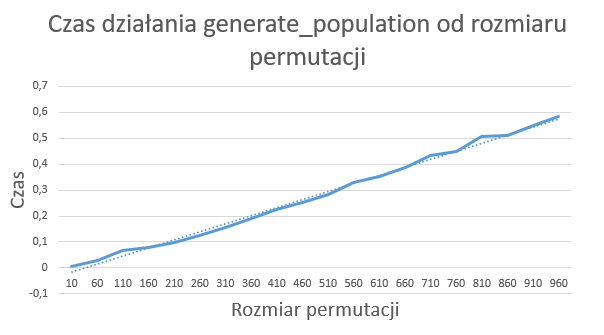
\includegraphics[scale=0.75]{GeneratePopulation.png}
    \centering
    \caption{Zależność czasu działania metody GeneratePopulation od rozmiaru permutacji}
    Przewidywana złożoność: $O(n)$ \\
    Złożoność wynikająca z testów: $O(n)$ \\
  \end{figure}
  \begin{figure}[H]
    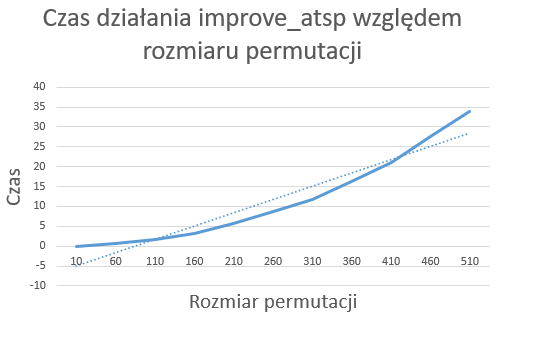
\includegraphics[scale=0.75]{ImproveAtsp.png}
    \centering
    \caption{Zależność czasu działania metody ImproveAtsp od rozmiaru permutacji}
    Przewidywana złożoność: $O(n^2*logn)$ \\
    Złożoność wynikająca z testów: Przypominająca $O(n^2)$ \\
    Należy zauważyć, iż przeprowadzana analiza jest dla przypadku worst-case, stąd mogą wystąpić rozbieżności między faktyczną, a przewidywaną złożonością.
  \end{figure}
  \begin{figure}[H]
    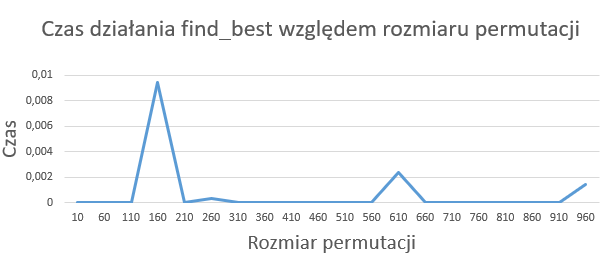
\includegraphics[scale=0.75]{FindBest.png}
    \centering
    \caption{Zależność czasu działania metody FindBest od rozmiaru permutacji}
    Przewidywana złożoność: $O(1)$ \\
    Złożoność wynikająca z testów: $O(1)$ \\
  \end{figure}
  \begin{figure}[H]
    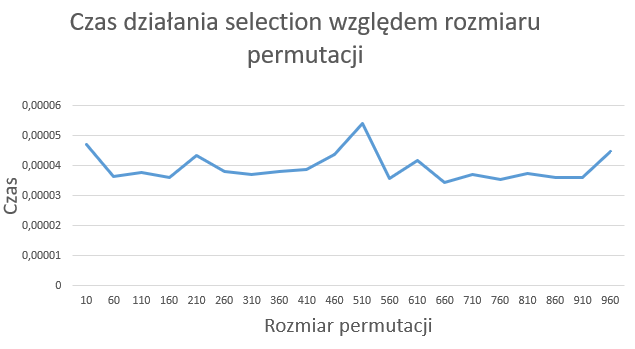
\includegraphics[scale=0.75]{Selection.png}
    \centering
    \caption{Zależność czasu działania metody Selection od rozmiaru permutacji}
    Przewidywana złożoność: $O(1)$ \\
    Złożoność wynikająca z testów: Przypominająca $O(1)$ \\
  \end{figure}
  \begin{figure}[H]
    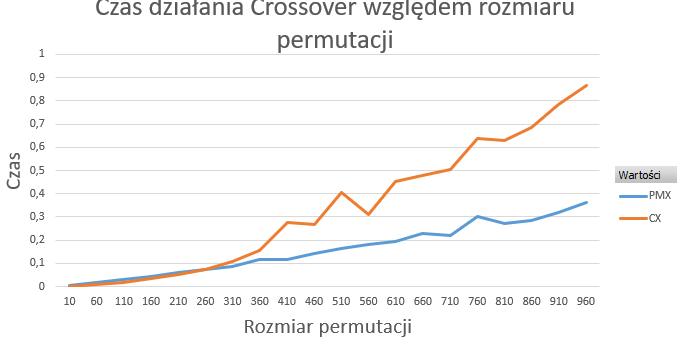
\includegraphics[scale=0.75]{Crossover.png}
    \centering
    \caption{Zależność czasu działania metody Crossover od rozmiaru permutacji}
    Przewidywana złożoność: $O(n)$ \\
    Złożoność wynikająca z testów: $O(n)$ \\
  \end{figure}
  \begin{figure}[H]
    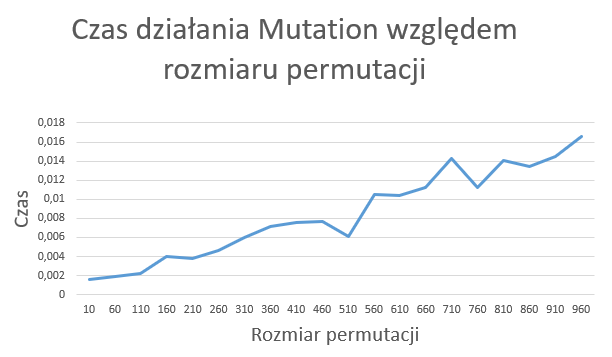
\includegraphics[scale=0.75]{Mutation.png}
    \centering
    \caption{Zależność czasu działania metody Mutation od rozmiaru permutacji}
    Przewidywana złożoność: $O(n)$ \\
    Złożoność wynikająca z testów:$O(n)$ \\
  \end{figure}
  \begin{figure}[H]
    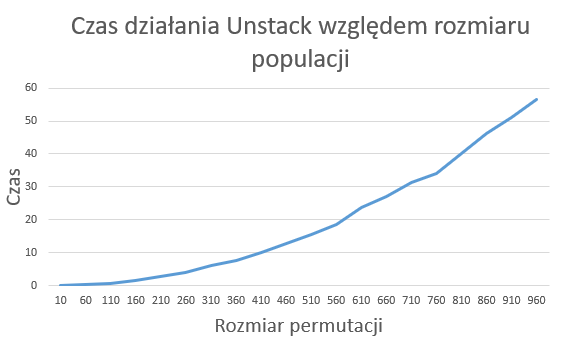
\includegraphics[scale=0.75]{Unstack.png}
    \centering
    \caption{Zależność czasu działania metody Unstack od rozmiaru permutacji}
    Przewidywana złożoność: $O(n*logn)$ \\
    Złożoność wynikająca z testów: $O(n^{2})$ \\
  \end{figure}
  \begin{figure}[H]
    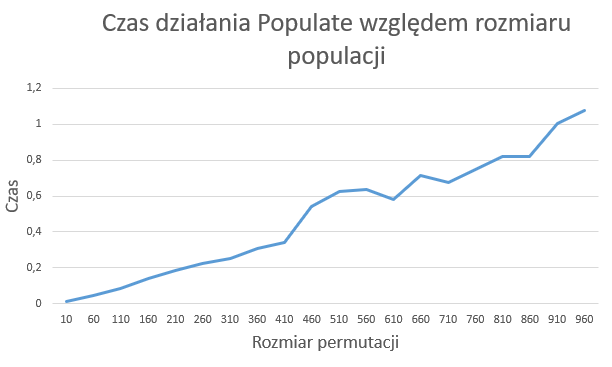
\includegraphics[scale=0.75]{Populate.png}
    \centering
    \caption{Zależność czasu działania metody Populate od rozmiaru permutacji}
    Przewidywana złożoność: $O(n*logn)$ \\
    Złożoność wynikająca z testów: Przypominająca $O(n)$ \\
  \end{figure}


  \textbf{Wniosek:}
  Zauważamy rozbieżność między teoretycznym wynikiem otrzymanym w wyniku analizy złożoności z praktycznym wynikiem otrzymanym w ramach testów.
  Wynika to z faktu, iż teoretyczny model zakłada podejście "worst-case", czyli podejście najgorszego przypadku, w którym metoda \textbf{Unstack()} wykonuje się w każdej iteracji pętli,
  jednakże w praktyce ów procedura wykonuje się stosunkowo rzadko. Ze względu na ten fakt zauważamy, iż w większości iteracji możemy pominąć wywołanie tej funkcji, co prowadzi do otrzymania
  liniowej złożoności obliczeniowej, którą faktycznie obserwujemy w przeprowadzonych testach.
